% !TEX root=main.tex

%\blue{How to use results from travelling salesman for trajectory recommendation?} 

%\noindent
The problem of recommending a trip over a set of POIs can be reduced to the classic travelling salesman problem (TSP)
if every POI is restricted to visit once.
However, in practice, we normally only visit a subset of these POIs,
which means results of TSP cannot be trivially used unless the subset of POIs is fixed.

%\noindent
%\blue{Not obvious how to directly use Christofides? Do we just find double visits and bypass?} 
%https://research.googleblog.com/2016/09/the-280-year-old-algorithm-inside.html

%\noindent
One well-known heuristic to approximately solve the TSP is the Christofides algorithm \citep{Christofides:1976}.
This algorithm finds a circuit that cost at most 1.5 times
of the optimal TSP solution, by constructing a minimum spanning tree and matching certain nodes, 
building the solution by simply bypassing repeated nodes.

Inspired by this, and recalling that the recommended trips by the classic Viterbi algorithm cannot avoid repeated visits,
we can first request a longer sequence using Viterbi and then skip repeated visits to form a trip, 
we keep asking for sequence with different length, until we cannot improve the resulting trip (with respect to the required length).
This algorithm is denoted as \textsc{Heuristic} in experiment.

\tikzstyle{state}=[shape=circle,draw=blue!50,fill=blue!20]
\tikzstyle{state2}=[shape=circle,draw=purple!50,fill=purple!20]
\tikzstyle{hiddenState}=[shape=circle,draw=gray!50,fill=gray!20,dashed]
\tikzstyle{specialState}=[shape=circle,double=red,draw=blue!50,fill=blue!20,dashed]
\tikzstyle{observation}=[shape=rectangle,draw=orange!50,fill=orange!20]
\tikzstyle{hiddenObservation}=[shape=rectangle,draw=gray!50,fill=gray!20,dashed]
\tikzstyle{lightedge}=[<-,thin]
\tikzstyle{mainstate}=[state,thick]
\tikzstyle{mainedge}=[<-,thick]

\begin{figure*}[!h]
    \centering
    %\subfloat[Original prediction with loop (dashed).]{
    \resizebox{0.8\textwidth}{!}{
    \subfloat[Method {\sc Heuristic}.]{
    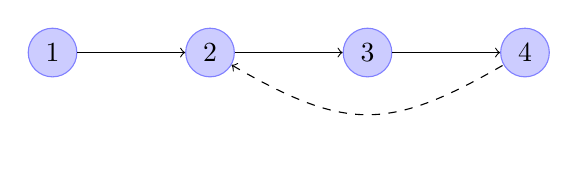
\begin{tikzpicture}[baseline=(s0.base)]
        % states
        \node[state] (s0) at (-2,2) {$1$};
        \node[state] (s1) at (0,2) {$2$}
            edge [<-] (s0);
        \node[state] (s2) at (2,2) {$3$}
            edge [<-] (s1);
        \node[state] (s3) at (4,2) {$4$}
            edge [<-] (s2);
        \draw [<-,dashed,bend right] (s1) to [looseness=1.25] (s3);

        \node[draw=none] at (0,1)  {};
    \end{tikzpicture}
    }%
    \qquad
    % \subfloat[Modified prediction with loop removed.]{
    % \begin{tikzpicture}[baseline=(s0.base)]
    %     % states
    %     \node[state] (s0) at (-2,2) {$1$};
    %     \node[state] (s1) at (0,2) {$2$}
    %         edge [<-] (s0);
    %     \node[state] (s2) at (2,2) {$3$}
    %         edge [<-] (s1);
    %     \node[state] (s3) at (4,2) {$4$}
    %         edge [<-] (s2);
    %     \draw [color=white,dashed,bend right] (s1) to [looseness=1.25] (s3);            
    % \end{tikzpicture}
    % }    
    \subfloat[Method {\sc List Viterbi}.]{
    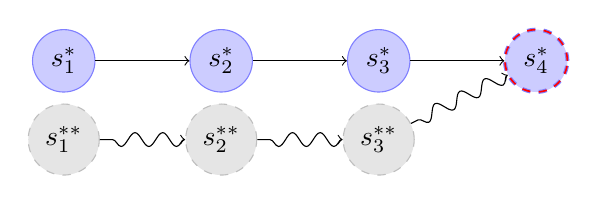
\begin{tikzpicture}[baseline=(s1.base)]
        % first-best
        \node[state] (s1) at (0,2)  {$s^*_1$};
        \node[state] (s2) at (2,2)  {$s^*_2$}            
            edge [<-] (s1);
        \node[state] (s3) at (4,2)  {$s^*_3$}            
            edge [<-] (s2);

        \node[hiddenState] (ss1) at (0,1) {{$s^{**}_{1}$}};                            
        \node[hiddenState] (ss2) at (2,1) {{$s^{**}_{2}$}}
            edge [<-,decorate,decoration={snake}] (ss1);                            
        \node[hiddenState] (ss3) at (4,1) {{$s^{**}_{3}$}}
            edge [<-,decorate,decoration={snake}] (ss2); 

        \node[specialState] (s4) at (6,2) {$s^*_4$}
            edge [<-] (s3)
            edge [<-,decorate,decoration={snake}] (ss3);
    \end{tikzpicture}
    }
    }

    \resizebox{0.5\textwidth}{!}{
    \subfloat[Method {\sc ILP}.]{
    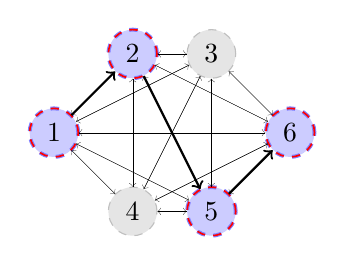
\begin{tikzpicture}[baseline=(s1.base)]
        % first-best
        \node[specialState] (s1) at (0,0)  {$1$};
        \node[specialState] (s2) at (1,1)  {$2$};
        \node[hiddenState]  (s3) at (2,1)  {$3$};
        \node[hiddenState]  (s4) at (1,-1) {$4$};
        \node[specialState] (s5) at (2,-1) {$5$};
        \node[specialState] (s6) at (3,0)  {$6$};

        %\node[draw=none] (juka) at (0,-1.5)  {};

        \draw [->,thick] (s1) to (s2);
        \draw [->,ultra thin] (s1) to (s3);
        \draw [->,ultra thin] (s1) to (s4);
        \draw [->,ultra thin] (s1) to (s5);
        \draw [->,ultra thin] (s1) to (s6);    

        \draw [->,ultra thin] (s2) to (s1);
        \draw [->,ultra thin] (s2) to (s3);
        \draw [->,ultra thin] (s2) to (s4);
        \draw [->,thick] (s2) to (s5);
        \draw [->,ultra thin] (s2) to (s6);    

        \draw [->,ultra thin] (s3) to (s1);
        \draw [->,ultra thin] (s3) to (s2);
        \draw [->,ultra thin] (s3) to (s4);
        \draw [->,ultra thin] (s3) to (s5);
        \draw [->,ultra thin] (s3) to (s6);    

        \draw [->,ultra thin] (s4) to (s2);
        \draw [->,ultra thin] (s4) to (s3);
        \draw [->,ultra thin] (s4) to (s1);
        \draw [->,ultra thin] (s4) to (s5);
        \draw [->,ultra thin] (s4) to (s6);    

        \draw [->,ultra thin] (s5) to (s2);
        \draw [->,ultra thin] (s5) to (s3);
        \draw [->,ultra thin] (s5) to (s4);
        \draw [->,ultra thin] (s5) to (s1);
        \draw [->,thick] (s5) to (s6);    

        \draw [->,ultra thin] (s6) to (s2);
        \draw [->,ultra thin] (s6) to (s3);
        \draw [->,ultra thin] (s6) to (s4);
        \draw [->,ultra thin] (s6) to (s5);
        \draw [->,ultra thin] (s6) to (s1);                    
    \end{tikzpicture}
    }%
    \qquad
    \subfloat[Method {\sc Greedy}.]{
    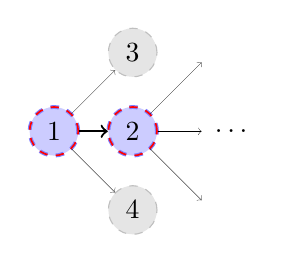
\begin{tikzpicture}[baseline=(s1.base)]
        % first-best
        \node[specialState] (s1) at (0,0)  {$1$};

        %\node[hiddenState] (s2) at (1,1.5)  {$2$};
        \node[hiddenState] (s3) at (1,1)  {$3$};
        \node[specialState] (s4) at (1,0)    {$2$};
        \node[hiddenState] (s5) at (1,-1) {$4$};
        %\node[hiddenState] (s6) at (1,-1.5)  {$6$};

        \node[draw=none] (s40) at (2,1)  {};
        \node[draw=none] (s41) at (2,0)     {};
        \node[draw=none] (s42) at (2,-1) {};

        \node[draw=none] (s411) at (2.25,0)     {$\ldots$};

        %\draw [->,ultra thin] (s1) to (s2);
        \draw [->,ultra thin] (s1) to (s3);
        \draw [->,thick] (s1) to (s4);
        \draw [->,ultra thin] (s1) to (s5);
        %\draw [->,ultra thin] (s1) to (s6);

        \draw [->,ultra thin] (s4) to (s40);
        \draw [->,ultra thin] (s4) to (s41);
        \draw [->,ultra thin] (s4) to (s42);
    \end{tikzpicture}
    }
    }
    
    %\caption{Example of heuristically removing loops. The nodes are numbered by the POI, with edges denoting order in the sequence. While the modified prediction removes the loop in the original sequence, it is necessarily at the expense of returning a path with fewer number of POIs.}
    \caption{Schematics of different algorithms to return a loop-free prediction.}
    \label{fig:heuristic}
\end{figure*}
